\section{Introduction}
\label{sec:intro}

Deep learning has developed rapidly in the last decade and become a crucial technique in various fields. 
However, neural networks would frequently make erroneous judgments in inference when encounter  the data  that differs greatly from their training data, which is known as out-of-distribution (OOD) data. This challenge is growing more prevalent and is particularly vital in safety-critical areas such as autonomous driving~\cite{filos2020can, janai2020computer} and medical diagnosis~\cite{pooch2020can}, which urges the development of effective OOD detection methods.

In practice, OOD data exhibits   large diversity and is difficult to identify~\cite{yang2021generalized_survey}.
Existing studies typically formulate OOD detection as a one-class classification task, utilizing prior knowledge. They~\cite{hendrycks2016msp, liu2020energy, yu2023block}  propose various priors, based on which  they further design scoring functions to distinguish OOD samples from ID samples.
For example, Hendrycks et al.~\cite{hendrycks2016msp}  observed that OOD samples always exhibit lower maximum softmax probabilities, and accordingly proposed using the maximal softmax probability output by a neural network as an OOD indicator. Liu et al.~\cite{liu2020energy} found that OOD samples usually have lower logits values, and based on this, an energy function was proposed for OOD detection.
Drawing from these precedents, it's clear that existing methods largely rely on the introduction of certain priors.  While some promising results highlight the effectiveness of these heuristics, a gap remains in meeting the practical requirements of real-world applications. Importantly, we note that the focus of these priors is narrowly concentrated on features and weights following global pooling, while the characteristics before the pooling layer are consistently ignored. Thus, we believe that finding and incorporating priors that can complement these existing focuses is essential, which will constitute the main contribution of our work.


In this study, we propose a novel prior, called \textbf{N}eural \textbf{A}ctivation \textbf{P}rior (NAP), for OOD detection. NAP characterizes our key observation that for channels before the global pooling layer in a fully trained neural network (illustrated to Figure~\ref{fig:pos}), a few neurons have a   significantly high probability to show 
a larger response when activated by in-distribution (ID) samples compared to OOD samples. An intuitive explanation for NAP is that channels in a model fully trained on an ID dataset play a role in detecting certain patterns in the input samples from the ID dataset. 
When such patterns are detected, a few neurons can be activated~\cite{hoefler2021sparsity}, resulting in larger responses. These large responses usually occur when the input sample is ID data, but when the input is OOD data, such responses are rarely observed. This is because the pattern that the neuron focuses on is unlikely to be present in the OOD data.
To verify our proposed prior, we employed DenseNet architecture~\cite{huang2017densely} on CIFAR-10~\cite{krizhevsky2009cifar} and Texture~\cite{cimpoi2014texture} datasets, analyzing mean and maximum within-channel activations before global pooling at the penultimate layer. Figure~\ref{fig:one} clearly demonstrates that ID samples exhibit significantly higher maximal activation values than OOD samples at equal average activation levels. Consequently, a series of methods, such as those in~\cite{hendrycks2016msp,sun2022knn,liu2020energy,liang2018odin_confi,lee2018maha_dist,sun2022dice,djurisic2022extremely,ahn2023line,sun2021react}, based on pooled activation values are unable to effectively distinguish these OOD samples, given the non-discriminative nature of their average activation values.

\begin{figure}[!t]
  \centering
  \begin{subfigure}{0.63\linewidth}
    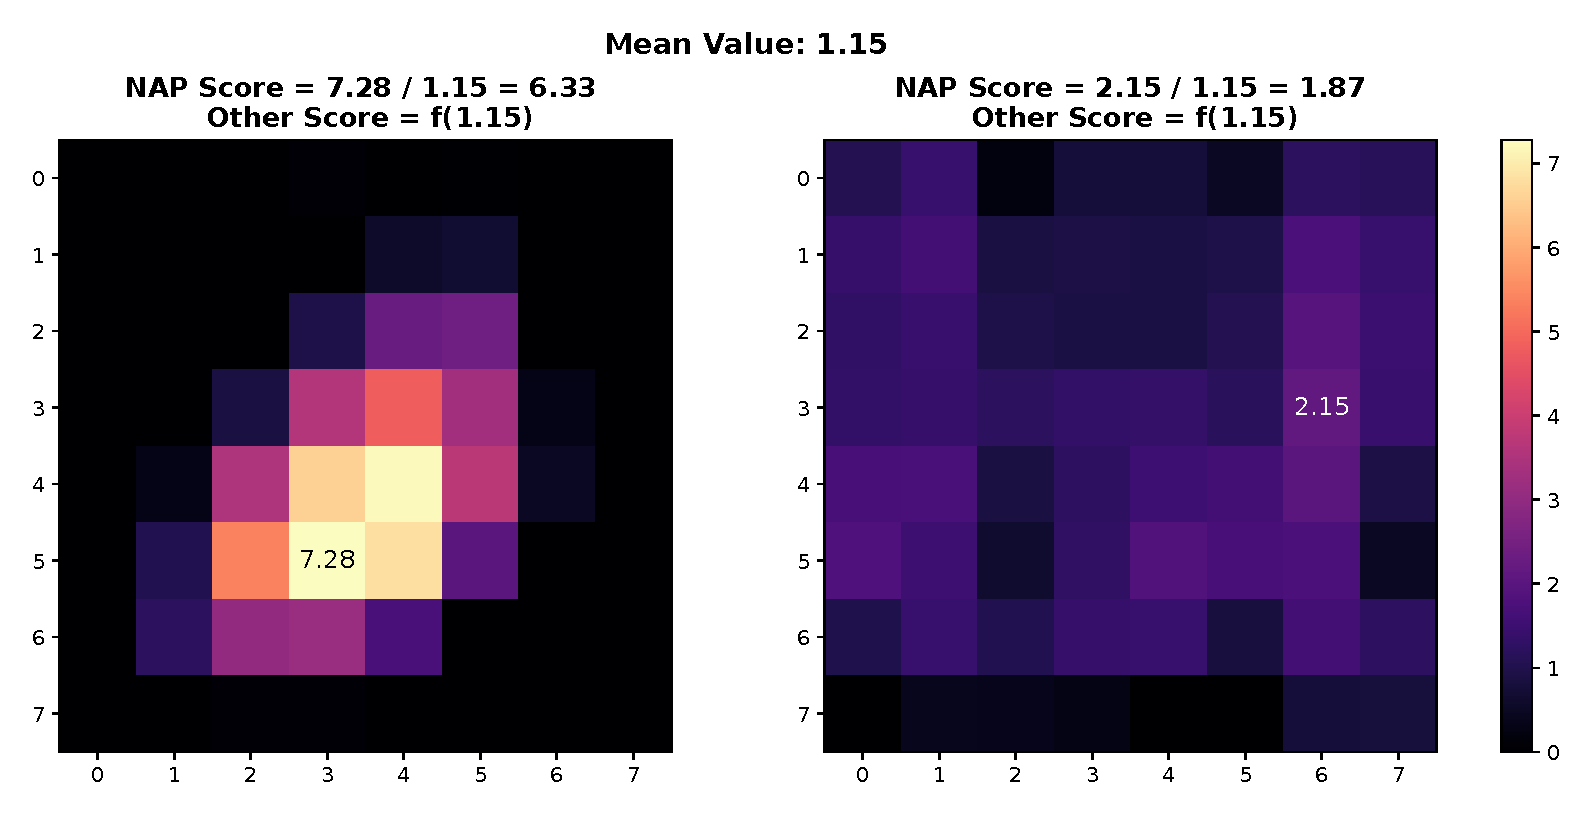
\includegraphics[width=0.99\linewidth]{eps/pair_24_channel_333_vis.eps}
    \caption{Activation Maps of ID and OOD samples.}
    \label{fig:activation_map}
  \end{subfigure}
  \hfill
  \begin{subfigure}{0.36\linewidth}
    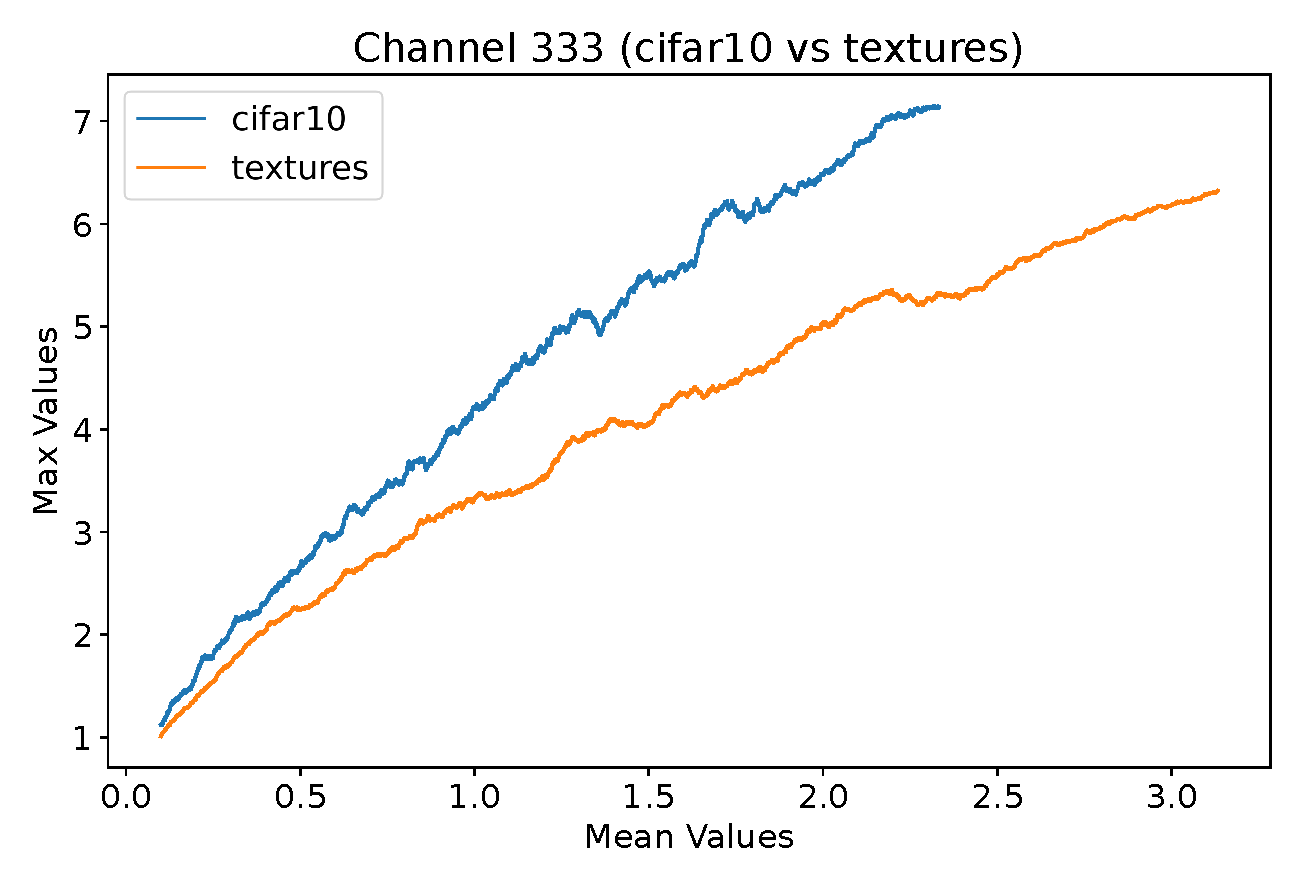
\includegraphics[width=0.99\linewidth]{eps/channel_333.eps}
    \caption{Activation distribution difference between ID data and OOD data.}
    \label{fig:activation_dis}
  \end{subfigure}
  \caption{\textbf{Global pooling leads to the neglect of distributional characteristics  of activation values within channels, thereby making it difficult to distinguish between ID and OOD samples.} (a) illustrates the activation value maps in the penultimate layer for in-distribution (ID) samples (left) and out-of-distribution (OOD) samples (right) within the same channel. In this layer, different channels typically focus on different semantic features. When a specific feature appears in an image, such as the central region in the left image, that location will have very high activation values. Although OOD samples lack these specific features, the model's unfamiliarity with OOD data leads to unpredictable activations, possibly causing weak noise activations (right image). This is detailed in \cite{sun2021react}. Existing methods often rely on pooled activation values for OOD detection. Thus, in (a), both ID and OOD samples have a mean channel activation of 1.15, making them indistinguishable by existing methods. However, the NAP score proposed in this paper can effectively distinguish between them. More examples like (a) are provided in the Appendix~\ref{appendix:vis}.
  (b) shows the activation distribution differences between ID and OOD data within the channel. The horizontal axis represents the average activation value, while the vertical axis represents the maximum activation value. Interestingly, at the same average activation level, ID data (CIFAR-10) shows significantly higher maximum activation values than OOD data (textures). This pattern is \textbf{not unique} to the \(333^\text{rd}\) channel but is observable in most channels, corroborating the phenomenon in (a).}
  \label{fig:one}
\end{figure}

% \begin{figure}[!t]
%   \centering
%   
\includegraphics[width=0.6\linewidth]{fig/channel_vis/channel_333.pdf}
%    \caption{\textbf{Activation distribution difference between ID data and OOD data inside channel.} This illustrates the difference in within-channel activation distribution between CIFAR-10~\cite{krizhevsky2009cifar} (ID data) and the Texture~\cite{cimpoi2014texture} (OOD data) datasets. The horizontal axis represents the average activation value of the channel, while the vertical axis shows the maximal activation value of the channel. Interestingly, at the same mean activation levels, the ID data (CIFAR-10) show significantly higher maximum activation values within the channel compared to the OOD data (Texture). It's important to note that this pattern is \textbf{not unique} to the \(333^\text{rd}\) channel but is observed across most channels.}
%    \label{fig:one}
%    % \vspace{-5pt}
% \end{figure}

It is worth noting that our proposed prior is orthogonal to that used in current OOD detection methods. In the OOD deteciton field, as shown in Figure~\ref{fig:pos}, existing methods~\cite{hendrycks2016msp,sun2022knn,liu2020energy,liang2018odin_confi,lee2018maha_dist,sun2022dice,djurisic2022extremely,ahn2023line,sun2021react} mainly focus on the outputs and weights of the neural network after global pooling, and use them to design scoring functions for OOD detection. In contrast, the prior we proposed is focus within the channels of the penultimate layer before global pooling. Since the information carried in our prior can be easily lost during the global pooling process, this demonstrates that our NAP  is essentially complementary to the priors used in current OOD detection studies. To this end, we would like to emphasize that the contribution of this paper would lie in how much improvement we can achieve by integrating our method with  existing approaches, rather than a direct comparison with existing methods in the field.


Furthermore, in this paper, we propose a simple yet effective scoring function for OOD detection based on our prior NAP. To be precise, our scoring function is based on the ratio of the maximal and averaged activation values within a channel.
The rationale behind the scoring function can be understood from two primary perspectives: conceptual inspiration from the Signal-to-Noise (SNR) and empirical validation.
On the conceptual front, inspired by the concept of SNR, we can consider the maximal activation value as signal strength, while the averaged activation value represents noise strength. Therefore, the ratio of the maximum to the average value can be used to measure the quality of information contained in the channel. On the empirical front, as shown in Figure~\ref{fig:one}, the ratio of the maximal and the  averaged values for ID samples is significantly higher than that of OOD data. Regarding practical deployment, as previously mentioned, our scoring function complements and, when multiplied with existing metrics, improves OOD detection, as depicted in Figure~\ref{fig:score-hists}. Also, it is noteworthy that this scoring function is a plug-and-play method, requiring no additional training, extra data, or reliance on pre-calculated statistical data from the training set, which makes it broadly applicable.

\begin{figure}[!t]
  \centering
  \begin{subfigure}{0.32\linewidth}
    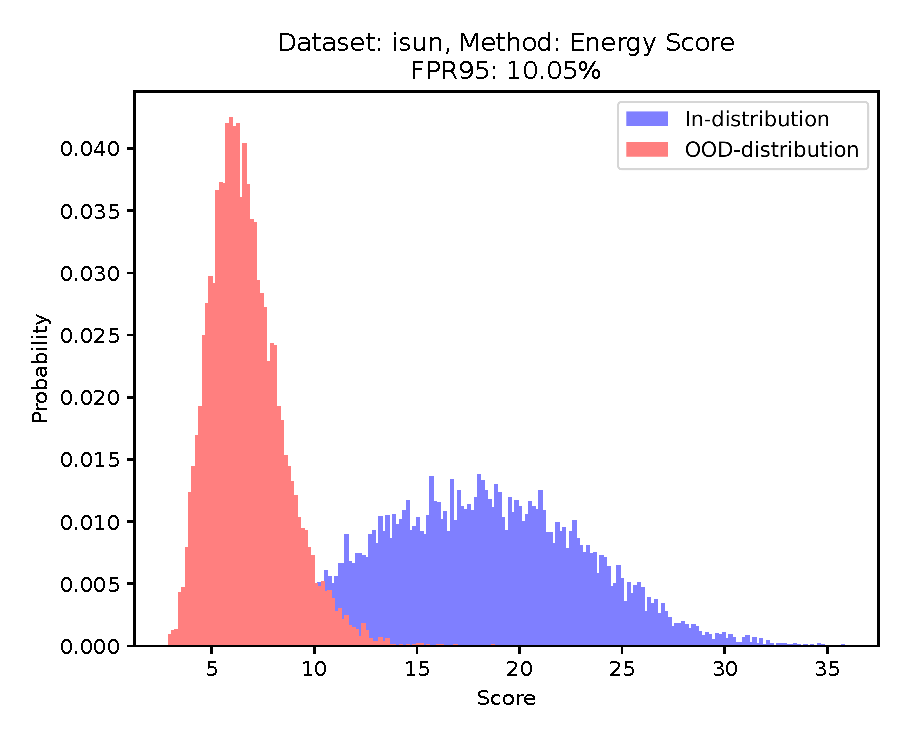
\includegraphics[width=0.99\linewidth]{eps/energy_isun.eps}
    \caption{Energy Score}
    \label{fig:hist-a}
  \end{subfigure}
  \hfill
  \begin{subfigure}{0.32\linewidth}
    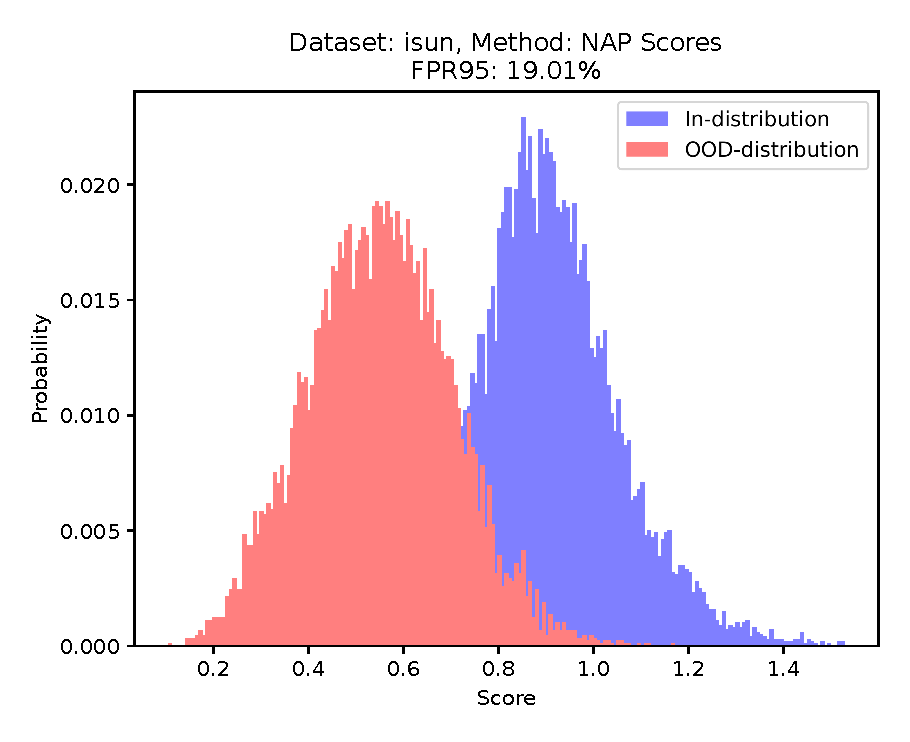
\includegraphics[width=0.99\linewidth]{eps/nap_isun.eps}
    \caption{NAP Score}
    \label{fig:hist-b}
  \end{subfigure}
  \hfill
  \begin{subfigure}{0.32\linewidth}
    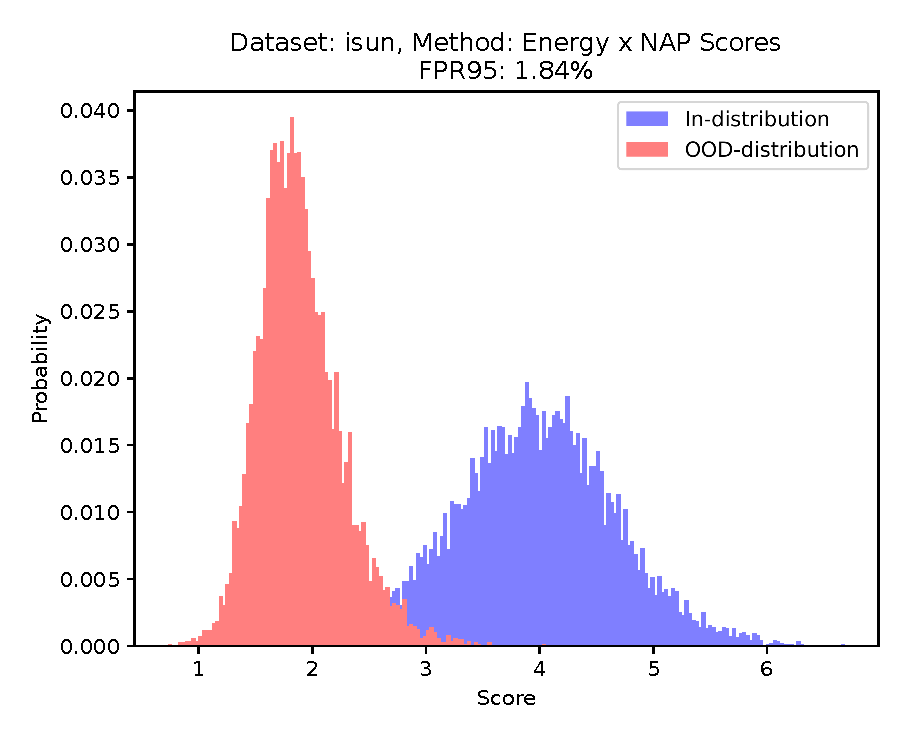
\includegraphics[width=0.99\linewidth]{eps/energy_nap_isun.eps}
    \caption{Energy $\times$ NAP Score}
    \label{fig:hist-c}
  \end{subfigure}
  \caption{\textbf{Score distribution visualization using DenseNet on CIFAR-10 (ID) and iSun (OOD)}
  The integration of (a) Energy Score and (b) NAP Score through multiplication yields the (c) Energy $\times$ NAP Score, demonstrating superior differentiation between ID and OOD datasets. The effectiveness of this approach is attributed to the orthogonal nature of the proposed NAP relative to conventional OOD detection methods exemplified by the Energy Score. This illustrates that a simple multiplicative combination with NAP enhances detection capability. Importantly, the objective is not merely to surpass the performance of the Energy Score itself, but to underscore the synergistic potential of NAP as a complementary enhancement to the Energy Score and similar method.}
  \label{fig:score-hists}
  % \vspace{-15pt}
\end{figure}

Experimental results show that our method achieves state-of-the-art performance on CIFAR-10~\cite{krizhevsky2009cifar}, CIFAR-100~\cite{krizhevsky2009cifar} and ImageNet datasets. Specifically, our method significantly reduces the false positive rate by 48.23\% (from 15.05 to 7.79) on the CIFAR-10 dataset~\cite{krizhevsky2009cifar}, a reduction of 37.89\% (from 41.40 to 25.71) on the CIFAR-100 dataset~\cite{krizhevsky2009cifar}, and a reduction of 16.26\% (from 35.66 to 29.86) on the ImageNet dataset. The large drop in FPR95 highlights the effectiveness of our approach in different environments.
The above experimental results demonstrate the power of our proposed prior. We believe that these findings will provide inspiration for other researchers and thus promote progress in the field of OOD detection.

Additionally, while convolutional neural networks (CNNs) are predominantly employed in OOD detection tasks, the advent of Transformer architectures~\cite{vaswani2017attention} and their variants has showcased substantial efficacy across a diverse array of applications. Motivated by this, we extend our method to ensure compatibility with Transformer models. The empirical evidence obtained from our experiments affirms the robustness of our approach, demonstrating its adaptability to various architectural paradigms.

In summary, our contributions are as follows:
\begin{itemize}
\item We introduce the Neural Activation Prior (NAP), a novel contribution to OOD detection. Uniquely, NAP is orthogonal to priors utilized in existing methods, offering a distinct and complementary perspective that paves the way for advanced OOD detection research.
\item Based on the proposed prior, we develop a simple yet effective OOD detection scoring function. 
% It is a plug-and-play approach that does not impair the model's inherent capabilities. 
It can be readily integrated with many existing OOD detection techniques, enhancing their ability to balance OOD detection with ID accuracy.
\item We demonstrate the state-of-the-art performance of our approach through extensive experiments across various datasets, including a reduction in FPR95 by up to 48.23\%. These results underscore the method's operational efficiency, simplicity of deployment, and overall efficacy. 
\item We extend the method to accommodate Transformer architectures. Experimental results are encouraging, validating the method's efficacy across various architectural designs.
\end{itemize}